\documentclass[crop,tikz]{standalone}
\usepackage{tikz}
\usepackage{xcolor}
\usetikzlibrary{arrows,decorations.pathmorphing,positioning}
% Helvetica for latex: https://www.sascha-frank.com/Fonts/Helvetica.html
\usepackage[scaled]{helvet}
\usepackage[T1]{fontenc}
\renewcommand\familydefault{\sfdefault}


\begin{document}

    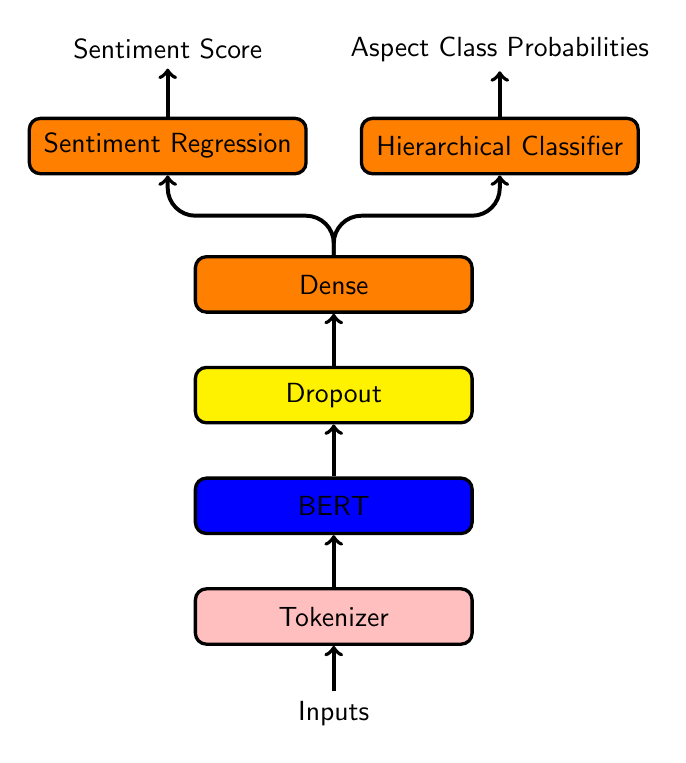
\begin{tikzpicture}

        % Text Nodes (without boxes)
        \node (inputs) at (0pt,-35pt) {Inputs};
        \node (sentimentscore) at (-60pt,205pt) {Sentiment Score};
        \node (aspectclassprobabilities) at (60pt,205pt) {Aspect Class Probabilities};

        % Model nodes
        \node (tokenizer) [draw, solid, minimum height=20pt, minimum width=100pt, xshift=00pt, fill=pink, fill opacity=1, very thick, rectangle, rounded corners] {Tokenizer};
        \node (bert) [draw, solid, minimum height=20pt, fill = blue, fill opacity=1,minimum width=100pt, xshift=00pt, yshift=40pt, very thick, rectangle, rounded corners] {BERT};
        \node (dropout) [draw, solid, minimum height=20pt, fill = yellow, fill opacity=1,minimum width=100pt, xshift=00pt, yshift=80pt, very thick, rectangle, rounded corners] {Dropout};
        \node (dense) [draw, solid, minimum height=20pt, fill = orange, fill opacity=1,minimum width=100pt, xshift=00pt, yshift=120pt, very thick, rectangle, rounded corners] {Dense};
        \node (sentimentregression) [draw, solid, minimum height=20pt, fill = orange, fill opacity=1,minimum width=100pt, xshift=-60pt, yshift=170pt, very thick, rectangle, rounded corners] {Sentiment Regression};
        \node (hierarchicalclassifier) [draw, solid, minimum height=20pt, fill = orange, fill opacity=1,minimum width=100pt, xshift=60pt, yshift=170pt, very thick, rectangle, rounded corners] {Hierarchical Classifier};

        % Arrows
        \draw[->, rounded corners=10pt, line width=0.5mm](inputs) -- (tokenizer);
        \draw[->, rounded corners=10pt, line width=0.5mm](tokenizer) -- (bert);
        \draw[->, rounded corners=10pt, line width=0.5mm](bert) -- (dropout);
        \draw[->, rounded corners=10pt, line width=0.5mm](dropout) -- (dense);
        \draw[->, rounded corners=10pt, line width=0.5mm](dense.north) -- ++(0,0.5) -|  (sentimentregression.south);
        \draw[->, rounded corners=10pt, line width=0.5mm](dense.north) -- ++(0,0.5) -|  (hierarchicalclassifier.south);
        \draw[->, rounded corners=10pt, line width=0.5mm](sentimentregression) -- (sentimentscore);
        \draw[->, rounded corners=10pt, line width=0.5mm](hierarchicalclassifier) -- (aspectclassprobabilities);

    \end{tikzpicture}
\end{document}